\documentclass[a4paper]{article}
\usepackage{geometry}
\geometry{left=2.5cm,right=2.5cm,top=2cm,bottom=2cm}
\usepackage{hyperref}
\usepackage{amsmath}
\usepackage{bm}
\usepackage{amsfonts,amssymb}
\usepackage{graphicx}
\usepackage{enumerate}
\usepackage{enumitem}  % Change the beginning order
\usepackage{booktabs}
\usepackage{float}

\title{ECMM719, Fluid Dynamics of the Atmospheres and Oceans\\
\textbf{EXAMINATION}}
\author{Qun Liu (Student No: 670016014)\\ \href{ql260@exeter.ac.uk}{ql260@exeter.ac.uk}
\\College of Enginerring, Mathematics and Physical Sciences}
\date{June, 2018}

\begin{document}

\maketitle

\textbf{SECTION A}

\begin{enumerate}[label=\textbf{\arabic*.}]
	\setcounter{enumi}{0}
	\item 
		\begin{enumerate}[label=\textbf{(\alph*)}]
			\setcounter{enumii}{0}
			\item Putting $\psi=\Psi\mathrm{e}^{i(kx+ly-\omega t)}$ into 
			$$\frac { \partial } { \partial t } \nabla ^ { 2} \psi + \beta \frac { \partial \psi } { \partial x } = 0$$
			gives
			$$ -i\omega(-k^2-l^2)+i\beta k=0,$$ 
			and thus the dispersion relation is
			$$ \omega=-\frac{\beta k}{k^2+l^2}.$$ 
			These kind of waves are Rossby waves.
			
			Phase speed in zonal diection is
			$$c^{x}_p=\frac{\omega}{k}=-\frac{\beta }{k^2+l^2},$$
			and group velocity in zonal direction is
			$$c^{x}_g=\frac{\partial \omega}{\partial k}=-\frac{\beta}{k^2+l^2}+\frac{2\beta k^2}{(k^2+l^2)^2}.$$
			Therefore, the relation between group and phase velocity is
			$$c _{ g }^{ x } = c _{ p }^{ x } + \frac{ 2\beta k ^ { 2} }{ \left( k ^ { 2} + l ^ { 2} \right)^{2} }.$$\\
			\vspace{0.5cm}
			\item 
			\begin{enumerate}[label=(\roman*)]
				\item The Boussinesq equations are valid for the fluid where the variation of density is very small compared to the mean density, and hence they are more
				likely to hold quantitatively in the ocean rather than atmosphere as the density variation is relative small in ocean.
				
				%Boussinesq equations ignores all the variations of density of fluid in momentum equation, except when associated with the gravitational term.
				\item 
				If the fluid is in geostrophic and hydrostatic balance, then the following equations
				\begin{equation*}
					\left.\begin{array} {c} { \frac {\mathrm{D} \bm v } {\mathrm{D} t } + f_ {0} \hat { \mathbf { k } } \times \bm v = - \nabla \phi + b \hat { \mathbf {k} } } ,\\ { \frac {\mathrm{D} b } {\mathrm{D} t } = 0}, \end{array} \right.
				\end{equation*}
				become
				%$$f_{0} \hat { \mathbf { k } } \times \bm v = - \nabla_z \phi,$$
				$$f_0v = \frac{\partial \phi}{\partial x},$$
				$$f_0u = -\frac{\partial \phi}{\partial y},$$
				$$\frac{\partial \phi}{\partial z}=b.$$
				
				In particular, the horizontal momentum equations can be rewritten as 
				$$ f_{0} \hat { \mathbf{k}} \times \bm u = - \nabla_z \phi,$$
				where $\bm u$ is horizontal wind and $\nabla_z$ is horizontal gradient.
				%and the vertical momentum equation is
				%$$\frac {\mathrm{D} w } {\mathrm{D} t}= -\frac{\partial \phi}{\partial z}+b$$
				Thus the horizontal gradient of buoyancy is (applying $\frac{\partial \phi}{\partial z}=b$)
				$$\nabla_z b = \frac{\partial b}{\partial x}+\frac{\partial b}{\partial y}=\frac{\partial }{\partial z}\left(\frac{\partial \phi}{\partial x} +\frac{\partial \phi}{\partial y}\right) = -\frac{\partial \nabla_z \phi}{\partial z}=-\frac{\partial f_{0} \hat { \mathbf{k}} \times \bm u}{\partial z}=-f_{0}\hat {\mathbf{k}} \times \frac{\partial \bm u}{\partial z},$$
				and hence it is associated with a vertical shear of the horizontal wind.
			\end{enumerate}
		\vspace{1cm}
		\item  
			\begin{subequations}\label{eq:linear_sw}
			\begin{equation}
			\frac { \partial u} {\partial t} - fv + \frac{\partial \Phi}{\partial x} = 0,
			\end{equation}	
			\begin{equation}
			\frac { \partial v}{\partial t} + fu + \frac{\partial \Phi} {\partial y} = 0,
			\end{equation}
			\begin{equation}
			\frac { \partial \Phi} {\partial t} + \Phi _ { 0} \left( \frac { \partial u} { \partial x} + \frac { \partial v} { \partial y} \right) = 0.
			\end{equation}
		\end{subequations}
		
		If the solutions for $u$, $v$ and $\Phi$ have the form 
		$$(u,v,\Phi) = \operatorname{Re} \{ (\hat{u},\hat{v},\hat{\Phi} )\exp [i(kx + l y - \omega t)]\}, $$
		then putting them into \eqref{eq:linear_sw} gives
		\begin{equation}\label{eq:matrix}
		\left(
		\begin{matrix}
		-i\omega& -f& ik\\
		f & -i\omega & il\\
		i\Phi_0k & i\Phi_0 l & -i\omega \\
		\end{matrix}
		\right)\left(
		\begin{matrix}
		\hat{u}\\
		\hat{v}\\
		\hat{\Phi}
		\end{matrix}
		\right)=0.
		\end{equation}
	
		To get non-trivial solutions, the determinant of matrix in \eqref{eq:matrix} should be 0, that is	
		$$-i\omega(-\omega^2+\Phi_0l^2)+f(-if\omega+\Phi_0lk)+ik(if\Phi_0l-\Phi_0k\omega)=0.$$
		Therefore, the  dispersion relation for this system is 
		\begin{equation}\label{eq:threeroots}
			\omega \left\{\omega^{ 2} - f^{2} - \Phi_{0} \left( k^{2} + l^{2} \right) \right\} = 0.
		\end{equation}
		
		The first root for dispersion relation \eqref{eq:threeroots} is
		%\begin{enumerate}[label=\textcircled{\arabic*}] 	%\end{enumerate}
		$\omega=0$, which gives a time-independent flow corresponding to geostrophic balance in \eqref{eq:linear_sw}. The other two roots are the solution of $$\omega^2 = f^{2} + \Phi_{0} \left( k^{2} + l^{2} \right),$$ and the corresponding waves are Poincare waves.
		\vspace{1cm}
		\item 
			\begin{enumerate}[label=(\roman*)]
			\item %	$$\frac { \text{D} q } { \text{D} t } = 0$$ 
				
			 If a parcel is displaced poleward (i.e. $y$ increase), the planetary vorticity $f(=f_0+\beta y)$ will increase. As $q$ is conserved and $q=\zeta +f$, so the relative vorticity $\zeta$ will decrease when the parcel moves northward ($f$ increased).
			 \item 
			 The poleward moving will lead to the decrease of relative vorticity, which gives rise to the velocity field that advects the parcels westward (shown in Figure \ref{fig:rossby}). As a consequence, the Rossby waves propagate to the west.
			 \begin{figure}[H]
			 	\centering
			 	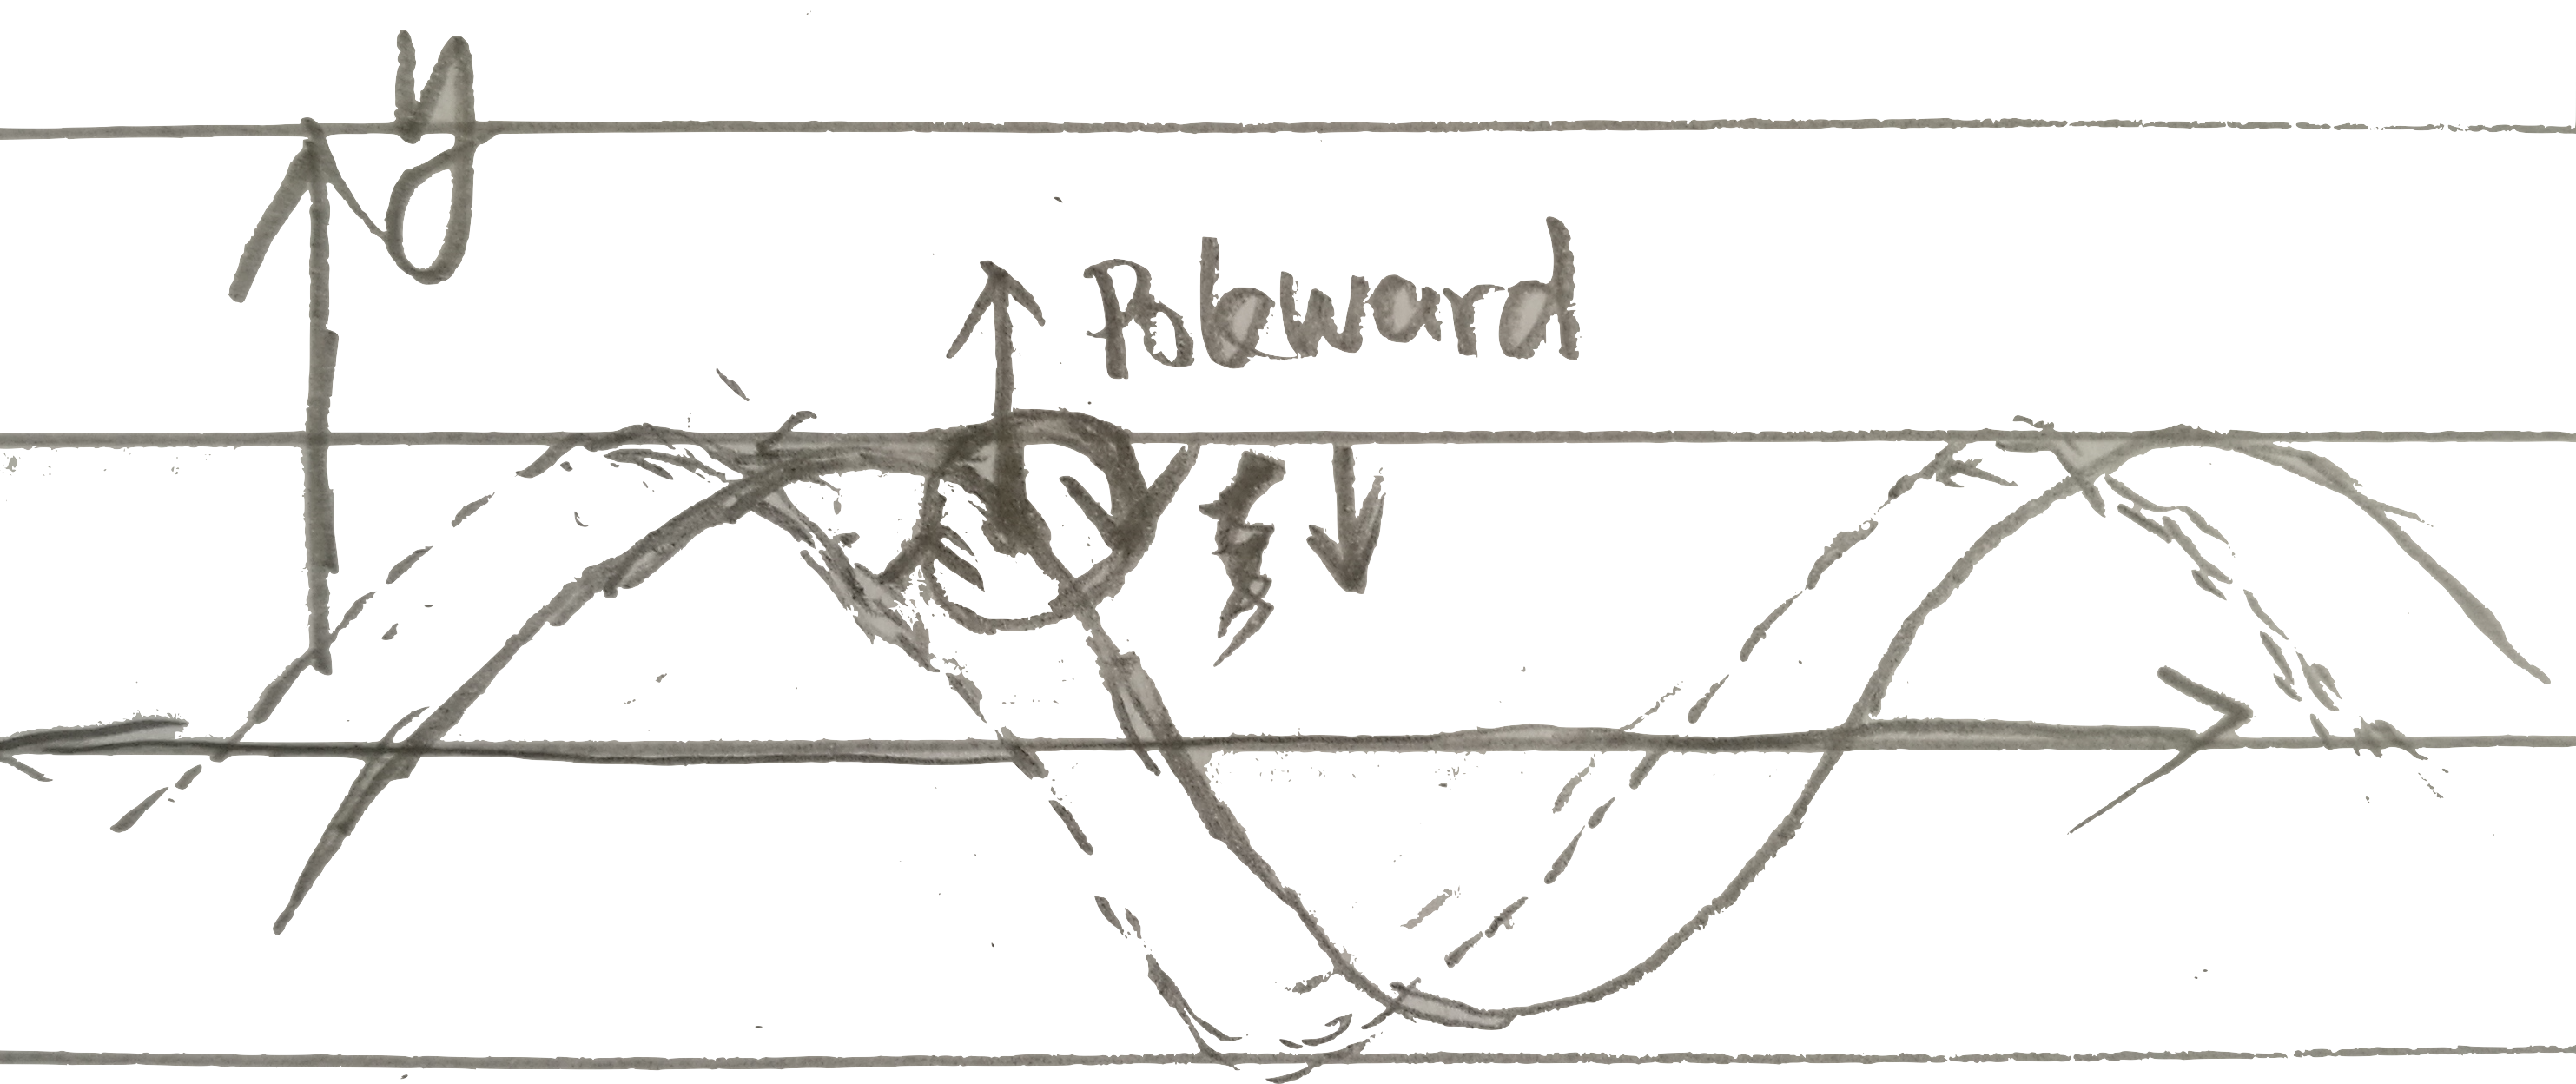
\includegraphics[width=0.4\linewidth]{./rossbywaveillustration.png}
			 	\caption{Illustration of parcel movement, and dash line indicates new position.}
			 	\label{fig:rossby}
			 \end{figure}
			\end{enumerate}
		\end{enumerate}
	\vspace{1.0cm}
	\newpage
%%%%%%%%%%%%%%%%%%%%%% SECTION B %%%%%%%%%%%%%%%%%%%%%%%%%%%%%%%%%%
 \textbf{SECTION B}

	\item 
		$$\left.\begin{array} { c } { \frac { D u } { D t } - f _ { 0} v = - \frac { \partial h } { \partial x } ,\quad \frac { D v } { D t } + f _ { 0} u = - \frac { \partial h } { \partial y } } \\ { \frac { D h } { D t } + h \left( \frac { \partial u } { \partial x } + \frac { \partial v } { \partial y } \right) = 0} \end{array} \right.$$
	
	%$$q = H \frac {\zeta + f_{ 0}} {h}$$
	%$$\zeta = (\partial v / \partial x - \partial u / \partial y )$$
	
		\begin{enumerate}[label=\textbf{(\alph*)}]
		\item From $q = H \frac {\zeta + f_{ 0}} {h}$, we obtain
		\begin{equation}\label{eq:qprime}
			Q' = H \frac {\zeta' + f_{ 0}} {h},
		\end{equation}
		where $Q'$ is a perturbation of $q$ and it is conserved, that is 
		\begin{equation}
			\frac{\partial Q'}{\partial t}+\bm u\cdot \nabla Q'=0.
			\label{eq:Q'_cons}
		\end{equation}

		Plugging $h = H + h^{ \prime }$ into \eqref{eq:qprime} gives
		\begin{equation}
			 Q'= H \frac{\zeta' + f_{ 0}} {H+h'} = \frac{\zeta' + f_{0}} {1+\frac{h'}{H}}
			 \label{eq:qprime2}
		\end{equation}
		In addition, $|h'|\ll H$ gives $\frac{h'}{H}\ll 1$. Considering $f_0\gg |\zeta'|$, hence \eqref{eq:qprime2} becomes
		\begin{equation}
		Q'\approx (\zeta' + f_{0}) \left( 1-\frac{h'}{H}\right) \approx f_0+\zeta'-\frac{f_0h'}{H}=f_0+q',
		\label{eq:qprime3}
		\end{equation}
		where	
		\begin{equation}
			q^{\prime } = \zeta^{\prime} - f_{0}\frac{h^{\prime }}{ H }.
			\label{eq:q'}
		\end{equation}
		Putting \eqref{eq:qprime3} and \eqref{eq:q'} into \eqref{eq:Q'_cons}, we obtain the linearised potential vorticity $q'$ satisfying 
		\begin{equation}
			\frac{\partial q'}{\partial t}=0.
		\end{equation}
		
		%	$$\zeta^{\prime } = \left( \partial v^{ \prime } / \partial x - \partial u ^ { \prime }/\partial y \right)$$
		
		
		\item 
		%$$\zeta^{\prime} = \nabla^{2}\psi$$
		%$$q^{\prime} = \nabla^{2}\psi - \frac{1}{L_{d} ^ {2}} \psi$$
		
		In the geostrophic balance, we have
		$$ f_0 v' = \frac{\partial h'}{\partial x}, \qquad f_0 u' = -\frac{\partial h'}{\partial y},$$
		
		and given that
		\begin{equation}\label{eq:psi_h'}
		\psi = \frac{ h'}{f_0},
		\end{equation}
		so the $u'$ and $v'$ become 
		$$v' = \frac{\partial \psi}{\partial x}, \qquad u' = -\frac{\partial \psi}{\partial y}.$$
		Therefore, $\zeta'$ could be written as
		\begin{equation}\label{eq:zeta'}
		\zeta'=\frac{\partial v'}{\partial x}-\frac{\partial u'}{\partial y}=\frac{\partial^2 \psi}{\partial x^2}+\frac{\partial^2 \psi}{\partial y^2}=\nabla ^2\psi.
		\end{equation}
		
		%According to \eqref{eq:psi_h'}, $$h'=\frac{f_0}{g}\psi,$$
		Put \eqref{eq:psi_h'} and \eqref{eq:zeta'} into \eqref{eq:q'}, we could get
		\begin{equation}\label{eq:q'_psi}
		q'=\zeta'-f_0\frac{h'}{H}= \nabla ^2\psi-\frac{f_0^2}{H}\psi=\nabla ^2\psi-\frac{1}{L_d^2}\psi,
		\end{equation}
		where $L_d=\sqrt{H}/f_0$.
		
		\item  Putting the \eqref{eq:q'_psi} into the initial potential vorticity and considering the flow will remain uniform in $y$ direction, we obtain 
		\begin{equation}\label{eq:psi_ctrl}
			\frac{\partial^2 \psi}{\partial x^2}-\frac{1}{L_d^2}\psi = \left\{ 
			\begin{array} 
			{cl} {-f_{0} h_{0}^{\prime } / H } & { x < 0} \\ 
			{f_{0} h_{0}^{\prime } / H } & { x > 0}
			\end{array} \right.
		\end{equation}
		
		Substituting the solution form
		$$\psi = \left\{ 
		\begin{array} {ll}{ - A \left( 1- e^{-x/B} \right) } & {x > 0} \\
		 {+ A \left( 1- e^{x/B} \right)} & {x < 0}
		 \end{array}
		 \right.$$
		 into \eqref{eq:psi_ctrl}, for $x<0$, we can get 
		 $$ \left\{ 
		 \begin{array} {ll} -\frac{A}{B^2}+\frac{A}{L_d^2}=0\\
		 -\frac{A}{L_d^2}=-\frac{f_0h_0'}{H}
		 \end{array}
		 \right. \Longrightarrow  \left\{ 
		 \begin{array} {ll} B=\pm L_d\\
		 A = \frac{f_0h_0'}{H}L_d^2 = \frac{h_0'}{f_0}
		 \end{array}
		 \right. $$
		 Considering the streamfunction and velocity can't be infinite at the $x=-\infty$, so we choose $B=L_d=\sqrt{H}/f_0$ when $x<0$. In addition, they also satisfy the solution for $x>0$. Hence, $$A=\frac{h_0'}{f_0},\qquad B= L_d=\sqrt{H}/f_0.$$
		\end{enumerate}
	
	\vspace{1cm}
	%%%%% New problem %%%%%%
	\item 
	
		\begin{enumerate}[label=\textbf{(\alph*)}]
			\item
			If the flow is in geostrophic balance, the Coriolis force term is balanced by the stress gradient, then we have
			\begin{subequations}
				\begin{equation}\label{eq:ek_geostro_v}
					fv_g = \frac{\partial \phi} {\partial x}, 
				\end{equation}
				\begin{equation}\label{eq:ek_geostro_u}
					fu_g = -\frac{\partial \phi} {\partial y},
				\end{equation}
			\end{subequations}
			where $v_g$ and $u_g$ are geostrophic velocities.
			Noticing that $f=f_0+\beta y$, $\frac{\partial \eqref{eq:ek_geostro_u}}{\partial x} + \frac{\partial \eqref{eq:ek_geostro_v}}{\partial y}$ gives
			$$f \left( \frac { \partial u_{ g } } { \partial x } + \frac { \partial v_{ g } } { \partial y } \right)+\beta v_g = -\frac{\partial^2 \phi} {\partial y\partial x} +\frac{\partial^2 \phi} {\partial x \partial y}=0,$$
			and therefore we could get		
			
			\begin{equation}\label{eq:eckman_geostrophic}
				f \left( \frac { \partial u_{ g } } { \partial x } + \frac { \partial v_{ g } } { \partial y } \right) = - \beta v_{ g }.
			\end{equation}
			
			Putting \eqref{eq:ek_geostro_v} and \eqref{eq:ek_geostro_u} back into (E1), that is 
				$$ (E1)\qquad -f v = -\frac { \partial \phi } { \partial x } + \frac { \partial \tau _ { x } } {\partial z } ,\quad f u = -\frac { \partial \phi } {\partial y } + \frac{ \partial \tau _ { y }} {\partial z },$$
			we have
			$$-f v = -fv_g + \frac { \partial \tau _ { x } } {\partial z } ,\quad f u = fu_g+ \frac{ \partial \tau _ { y }} {\partial z },$$
		    and then we can obtain
			$$ (E2)\qquad f\left( v_{g} - v \right) = \frac { \partial \tau _ { x } } { \partial z } ,\quad f \left(u - u_{g} \right) = \frac { \partial \tau _ {y} } {\partial z }.$$
			
			\item 
				
			Rewriting (E2) in the vector form gives
			\begin{equation}\label{eq:vector_eckman}
			\bm f\times (\bm u-\bm u_g) = \frac{\partial \bm\tau } { \partial z },
			\end{equation}
			where $\bm u=(u,v), \bm u_g=(u_g,v_g)$ and $ \bm \tau =(\tau_x, \tau_y)$.
			Integrating \eqref{eq:vector_eckman} from the bottom to top of the Eckman layer, we obtain
			\begin{equation}\label{eq:eckman_layer_transp}
			\bm f\times \bm M_{_a}=  \int_{-H_E}^{0} \frac{\partial \bm\tau } { \partial z }dz=\bm \tau_{_T}-\bm \tau_{_B},
			\end{equation} 
			where $\bm M_{_a}=\int_{-H_E}^{0} (\bm u -\bm u_{_g})dz$ is the agostrophic transport, and $\bm \tau_{_T}$ and $\bm \tau_{_B}$ are the wind stress at the top and bottom of Eckman layer respectively, with value $\bm \tau_{_T} = \bm \tau_0 = (\tau_{x0}, \tau_{y0})$ and $\bm \tau_B=0$. From \eqref{eq:eckman_layer_transp} we could get
			$$\bm M_{_a}= \frac{1}{f}\bm {k}\times (\bm \tau_{_T}-\bm \tau_{_B}),$$
			$$\Longrightarrow \bm M_{a}= \frac{1}{f}\bm {k}\times \bm \tau_{_T}, $$ which is at the right angle of surface stress.
			
			\item 
			$$w_{ E } = \left[ \frac { \partial } { \partial x } \left( \frac { \tau_{ y 0} } {f} \right) - \frac { \partial } { \partial y } \left( \frac { \tau_ { x0} } {f} \right) \right] - \int_{- HE }^{ 0} \frac { \beta } { f } v_{ g } d z$$
			
			
			The mass continuity is 
			\begin{equation}\label{eq:mass}
			\frac { \partial u } { \partial x } + \frac { \partial v } { \partial y } + \frac { \partial w } { \partial z } = 0.
			\end{equation}
			Integrating the mass continuity equation over the depth of the Ekman
			layer, we have
			$$\int_{-H_{E}}^{0} \frac{ \partial w}{\partial z} \mathrm{d}z =-\int_{-H_{E}}^{0} \left( \frac { \partial u } { \partial x } + \frac { \partial v} { \partial y }\right)dz = 0-w_E=-w_E,$$
			hence
			\begin{equation}\label{eq:w_e}
				w_E = \int_{-H_{E}}^{0} \left( \frac { \partial u } { \partial x } + \frac { \partial v} { \partial y }\right)dz
			\end{equation}
			
			From (E2) we could get
			$$u = u_g+ \frac{1}{f} \frac{\partial \tau_y}{\partial z} , \qquad v = v_g -\frac{1}{f} \frac{\partial \tau_x}{\partial z}. $$
			Combining them with mass continuity equation \eqref{eq:mass} gives
			$$\frac { \partial u } { \partial x } + \frac { \partial v } { \partial y } = \left[\frac{\partial }{\partial x} \left( \frac{1}{f}\frac{\partial \tau_y}{\partial z} \right) - \frac{\partial }{\partial y} \left( \frac{1}{f}\frac{\partial \tau_x}{\partial z} \right) \right] + \frac { \partial u_g } { \partial x } + \frac { \partial v_g } { \partial y }.$$
			
			From \eqref{eq:eckman_geostrophic} we obtain 	
			$$\frac { \partial u_g } { \partial x } + \frac { \partial v_g } { \partial y } = -\frac{\beta v_g}{f},$$
			hence
			$$\frac { \partial u } { \partial x } + \frac { \partial v } { \partial y } = \left[\frac{\partial }{\partial x} \left( \frac{1}{f}\frac{\partial \tau_y}{\partial z} \right) - \frac{\partial }{\partial y} \left( \frac{1}{f}\frac{\partial \tau_x}{\partial z} \right) \right] -\frac{\beta v_g}{f} = \frac { \partial } {\partial z} \left[\frac{\partial }{\partial x} \left(\frac{\tau_y}{f}\right)- \frac{\partial }{\partial y}\left(\frac{\tau_x}{f}\right) \right]  -\frac{\beta v_g}{f}.$$
			
			Integrating the above equation gives
			$$\begin{aligned}
			 \int_{-H_{E}}^{0} \left( \frac { \partial u } { \partial x } + \frac { \partial v} { \partial y }\right)dz 	&= \int_{ -H_E }^{0}\frac { \partial } {\partial z} \left[\frac{\partial }{\partial x} \left(\frac{\tau_y}{f}\right)- \frac{\partial }{\partial y}\left(\frac{\tau_x}{f}\right) \right] dz - \int_{- H_E }^{ 0} \frac { \beta v_{ g }  } { f } d z \\
			 & =\left[ \frac { \partial } { \partial x } \left( \frac { \tau  _ { y 0} } { f } \right) - \frac { \partial } { \partial y } \left( \frac { \tau _ { x0} } { f } \right)\right]- \int_{- H_E }^{ 0} \frac { \beta v_{ g }  } { f } d z.\\
			\end{aligned} $$
			Hence, \eqref{eq:w_e} becomes
			$$w_E=\left[ \frac { \partial } { \partial x } \left( \frac { \tau  _ { y 0} } { f } \right) - \frac { \partial } { \partial y } \left( \frac { \tau _ { x0} } { f } \right)\right]-\int_{- H_E }^{ 0} \frac { \beta v_{ g }  } { f } d z $$
			
			\item Cross-differentiating equations (E1) gives
			$$f\left(\frac { \partial u}{\partial x } + \frac { \partial v}{ \partial y }  \right) =  - \beta v+\frac { \partial } {\partial z} \left( \frac{\partial \tau_y}{\partial x} - \frac{\partial \tau_x}{\partial y} \right), $$
			and combining the mass continuity equation \eqref{eq:mass}, we obtain
			$$\beta v = \frac { \partial } {\partial z} \left( \frac{\partial \tau_y}{\partial x} - \frac{\partial \tau_x}{\partial y} \right) +f\frac{\partial w}{\partial z}.$$
			
			Integrating the above equation from the ocean bottom $H_o$ to the surface and considering the vertical velocity is zero at bottom and surface of the ocean, we obtain
			
			$$ \begin{aligned}
			\int_{-H_o}^0 \beta v d z & = \int_{-H_o}^0 \frac { \partial } {\partial z} \left( \frac{\partial \tau_y}{\partial x} - \frac{\partial \tau_x}{\partial y} \right) dz + \int_{-H_o}^0 f\frac{\partial w}{\partial z}dz\\
			&= \frac { \partial \tau_{y0} } { \partial x } - \frac { \partial \tau_{ x 0} } { \partial y }.
			\end{aligned} $$

		\end{enumerate}	
	
\end{enumerate}

\end{document}
